\section{Generalizations : Outlier and LAD}
\subsection{Implementation and experiments}

We implemented a function {\tt LADRegression} that, given a maximum degree $M$ and a regularization parameter $\lambda$ compute the polynomial ridge regression. Mathematically, we want to minimize in $w$ the following expression:
\begin{equation*}
    \sum_i |(A\mathbf{w} - \mathbf{y})_i|^2 + \lambda \|\mathbf{w}\|^2
\end{equation*}
Where, in the case of polynomial regression, $w$ are the polynomial coefficients, $x$ the vector of data points and:
\begin{equation*}
    A_{i,j} = x_i^{j-1}, \qquad \forall \, 1 \leq i \leq n, \, 1 \leq j \leq M+1
\end{equation*}

We experimented the LAD regression on the simple data from Bishop's Figure 1.4. In order to have compelling results, we are using an improved gradient descent with randomization. Indeed, it allows us to avoid meaningless local minima, even if we are not guaranteed to converge to the global one.

Figure~\ref{fig:lad1} represents the results we obtained when varying parameters $M$ and $\lambda$. The two first regression are pure L1 ($\lambda = 0$), and the two lower ones allow us to study the influence of parameter $\lambda$. We can study here the difference between a L1 error and a L2 one.
\begin{itemize}
    \item With a L1 error, the fitted curve tends to go through several points exactly.
    \item With a L1 error, the fitted curve is ``allowed'' to be far from a few points: this is promising to deal with outliers.
    \item With the sensitivity of the solution to the parameter $\lambda$ is the same as in the L2 case: when $\lambda$ is too high, the polynomial coefficients become very small.
\end{itemize}

\begin{figure}[h]
  \centering
 \includegraphics[width=10.3cm]{../Figures/Q4/LAD1.png}
\caption{LAD regression for various $M$ and $\lambda$. The green curve represents the original $\sin$ function used to generate the red datapoints}
\label{fig:lad1}
\end{figure}



\subsection{New dataset and grid-search}
We use the same method with the new dataset. But this time, we are given a validation set. We use it to optimize the value of the parameters $M$ and $\lambda$, using the grid-search technique as before.

Figure~\ref{fig:lad2} shows four different sets of parameters and the corresponding regressions and validation errors. The first one is the most simple case of pure affine least-square regression, good to compare the validation error. We  immediately see that the outlier is dealt with a more efficiently than before, and the validation MSE is very good. The second and third graphs represent solutions with higher $M$. They are not as good, as a higher degree allow the curves to be closer to the outlier and results in a bad validation set MSE.
The result of the grid-search for best parameters is plotted in the last figure, with $M=1$ and $\lambda = 1.0$ (surprisingly, 1.0 is better than, say, 1.1 and 0.9). We can see that we are very close to what we want, and we expect a good error on the testing set.

Indeed, computing the MSE on the testing set with $M=1$ and $\lambda = 1$ gives a mean error of $0.1115$, which is a lot better than the $2.76$ given by Ridge regression.

\begin{figure}[h]
  \centering
 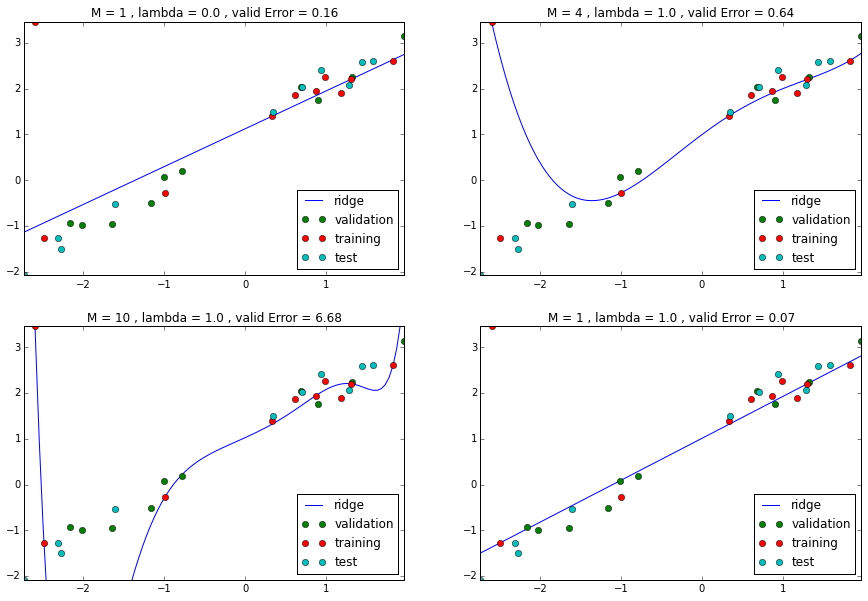
\includegraphics[width=10.3cm]{../Figures/Q4/lad2.png}
\caption{LAD regression for various $M$ and $\lambda$. The fit is done on the training set (with one outlier) and the error is computed on the validation set.}
\label{fig:lad2}
\end{figure}

\subsection{Application on BlogFeedback data}
We recompute the same graphs as before: Figure~\ref{fig:grid2} represent the grid-search of parameter $\lambda$. The best value is $10^{2.97}$.
\begin{figure}[h]
  \centering
 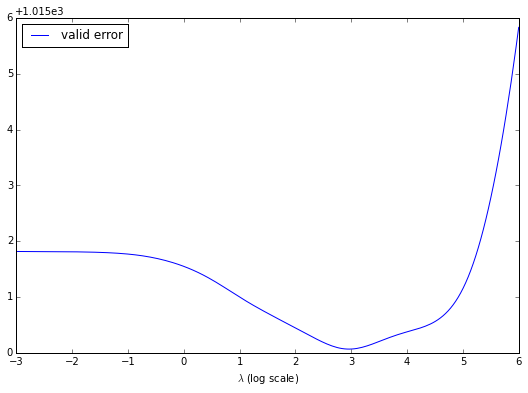
\includegraphics[width=8cm]{../Figures/Q4/grid.png}
\caption{LAD : Grid-search for parameter $\lambda$. The y-axis is the mean-squared validation error and the x-axis is $\log_{10}(\lambda)$ .}
\label{fig:grid2}
\end{figure}

Here is a summary of our mean-square error results using $\lambda = 10^{2.97}$ with our linear model:
\begin{center}
  \begin{tabular}{| c  | c |c |}
    \hline
 Learning set MSE & Validation set MSE &  Test set MSE \\ \hline
 880.59  &  1016.82 & 899.95 \\
    \hline
  \end{tabular}
\end{center}
The results are comparable with the ridge ones. We are doing slightly worse on the training and testing sets, and slightly better on the validation set.

\subsection{Interpretations and conclusion}
We have seen that LAD clearly outperforms ridge when in presence of a single outlier. On the other hand, on a real dataset with enough data, the noise is often ``white'' and outliers compensate each-other. As a consequence, ridge and LAD are similar. In this case, we actually have a slight preference for ridge, as it as good probabilistic guarantees. (In the case of gaussian noise, it is the right estimator).

Therefore, our conclusion is the following:
\begin{itemize}
    \item On a small to medium dataset with outliers that are hard to pre-remove: prefer LAD
    \item On a large dataset where the Law of Large Numbers applies and outliers are not as important anymore, or on any dataset where there are no outliers: prefer ridge, as we have good probabilistic guarantees and a closed form for the solution.
\end{itemize}
